\documentclass{ctexart}

\usepackage{ctex}
\usepackage{tikz}
\usepackage{amsmath}
\usepackage{xltxtra}
\usepackage{xcolor}
\usepackage{hyperref}
\usepackage{subfigure}
\usepackage{graphicx}
\usepackage[a4paper,left=1.25in,right=1.25in,top=1in,bottom=1in]{geometry}

\title{Notes on Numerical Analysis \\ 数值分析}

\author{Qinghai Zhang}

\begin{document}

\maketitle
\tableofcontents
\addcontentsline{toc}{section}{Solving Nonlinear Equations 求解非线性方程组}
\addcontentsline{toc}{section}{Polynomial Interpolation 多项式插值}
\addcontentsline{toc}{section}{Splines 样条}
\addcontentsline{toc}{section}{Computer Arithmetic 计算机算法}
\addcontentsline{toc}{section}{Approximation 近似值}
\addcontentsline{toc}{section}{Numerical Integration and Differentiation 数值积分与微分}
\addcontentsline{toc}{section}{附录}

\section{Solving Nonlinear Equations 求解非线性方程组}
\subsection{The bisection method 二分法}
二分法通过重复地将间隔减小到根存在的半间隔来求连续函数 f: R $\rightarrow$ R.

\fbox{\begin{minipage}{12cm}
    \textbf{Input}: $f:[a,b] \rightarrow R, a \in R, b \in R, M \in N^+, \delta \in R^+, \epsilon \in R^+$
    
    \textbf{Preconditions(前置条件)}: $f \in C[a,b], sgn(f(a)) \ne sgn(f(b))$
    
    \textbf{Output}: c, h, k
    
    \textbf{Postconditions(终止条件)}: |f(c)| < $\epsilon$ or |h| < $\delta$ or k = M
    
\end{minipage}}
\begin{verbatim}
1 u <- f(a)
2 v <- f(b)
3 for k = 1:M do
4     h <- b-a
5     c <- a+h/2
6     w <- f(c)
7     if |h| < delta or |w| < epsilon Then
8        break
9     else if sgn(w) =! sgn(u) then
10         b <- c  v <- w
11         else
12         a <- c  u <- w
13    end
14 end
\end{verbatim}

\subsection{The signature of an algorithm 算法的签名}
\textbf{Definition 1.2. 算法是一个逐步的过程,它将一组值作为输入,并生成一组值,作为输出。}

(An algorithm is a step-by-step procedure that takes some set of values as its input and produces some set of values as its output.)

\textbf{定义 1.3. 先决条件是在执行算法之前保持输入的条件。}

(A precondition is a condition that holds for the input prior to the execution of an algorithm.)

\textbf{定义 1.4. 后置条件是在执行算法后对输出有效的条件}

(A postcondition is a condition that holds for the output after the execution of an algorithm.)

\textbf{定义 1.5. 算法的签名包括其输入、输出、先决条件、后置条件以及如何处理违反先决条件的输入参数。}

(The signature of an algorithm consists of its input, output, preconditions, postconditions, and how input parameters violating preconditions are handled.)

\subsection{Proof of correctness and simplification of algorithms 算法的正确性证明和简化}
\textbf{定义 1.6. 不变量是在算法执行期间保持不变的条件。}

(An invariant is a condition that holds during the execution of an algorithm.)

\textbf{定义 1.7. 如果变量是在循环中初始化的,则该变量是临时变量或从循环中派生的变量。如果变量在循环之前初始化,并且其值在不同迭代期间发生变化,则变量对于循环是持久的或主要的。}

(A variable is temporary or derived for a loop if it is initialized inside the loop. A variable is persistent or primary for a loop if it is initialized before the loop and its value changes across different iterations.)

\textbf{定义 1.8. 算法1.1中的不变量是什么?a、b、c、h、u、v、w代表哪些量?其中哪些是主要的?以下哪些变量是临时变量?绘制图片以说明这些变量的寿命。}

(What are the invariants in Algorithm 1.1? Which quantities do a, b, c, h, u, v, w represent? Which of them are primary? Which of these variables are temporary? Draw pictures to illustrate the life spans of these variables.)

\textbf{定义 1.9. 一种简化的二等分算法。}

(A simplified bisection algorithm.)

\fbox{\begin{minipage}{12cm}
    \textbf{Input}: $f:[a,b] \rightarrow R, a \in R, b \in R, M \in N^+, \delta \in R^+, \epsilon \in R^+$
    
    \textbf{Preconditions(前置条件)}: $f \in C[a,b], sgn(f(a)) \ne sgn(f(b))$
    
    \textbf{Output}: c, h, k
    
    \textbf{Postconditions(终止条件)}: |f(c)| < $\epsilon$ or |h| < $\delta$ or k = M
    
\end{minipage}}
\begin{verbatim}
1 h <- b-a
2 u <- f(a)
3 for k = 1:M do
4     h <- h/2
5     c <- a+h
6     w <- f(c)
7     if |h| < delta or |w| < epsilon Then
8        break
9     else if sgn(w) = sgn(u) then
10         a <- c
11    end
12 end
\end{verbatim}

\subsection{Q-order convergence Q阶收敛}
\textbf{定义 1.10. (Q-order convergence)收敛序列$\{x_n\}$收敛于L,若:}

\[
\lim_{n \rightarrow \infty} \frac{|x_{n+1} - L|}{|x_n - L|^p} = c > 0; (1.1)
\]

\textbf{常数c称为渐近因子。特别地,当p=1时,$\{x_n\}$具有Q-线性收敛性,而当p=2时,具有Q-二次收敛性。}

(A convergent sequence ${x_n}$ is said to converge to L with Q-order p (p $\ge$ 1),the constant c is called the asymptotic factor. In particular, ${x_n}$ has Q-linear convergence if p = 1 and Q-quadratic convergence if p = 2.)

\textbf{定义 1.11. 迭代序列$\{x_n\}$被称为线性收敛到L,如果:}

\[\exists c \in (0,1),\exists d > 0, s.t. \forall n \in N, |x_n - L| \le c^nd.   (1.2)
\]
\textbf{对于一个收敛到L的序列$\{x_n\}$,其收敛阶数是所有满足$p \in R^+$中最大的那个p。}
\[
\exists c > 0,\exists N \in N s.t. \forall n > N,|x_{n+1}-L| \le c|x_n-L|^p.  (1.3)
\]
\textbf{特别的,如果p=2,则$\{x_n\}$二次收敛}

(A sequence of iterates $\{x_n\}$ is said to converge linearly to L if: For a sequence $\{x_n\}$ that converges to L, its order of convergence is the maximum $p \in R^+$ satisfying.In particular, $\{x_n\}$ converges quadratically if p = 2.)

\textbf{定义 1.12. (单调序列定理 Monotonic sequence theorem)每个有界单调序列都是收敛的。}

(Every bounded monotonic sequence is convergent.)

\textbf{定义 1.13. (二分法的收敛性 Convergence of the bisection method).对于满足$sgn(f(a_1)) \ne sgn(f(b_2))$的连续函数$f:[a_0,b_0]\rightarrow R$,二分法中的迭代序列线性收敛于渐近因子$\frac{1}{2}$}
\[
\lim_{n \rightarrow \infty} a_n = \lim_{n \rightarrow \infty} b_n = \lim_{n \rightarrow \infty} c_n = \alpha, (1.4)
\]
\[
f(\alpha) = 0, (1.5)
\]
\[
|c_n - \alpha| \le 2^{-(n+1)}(b_0 - a_0), (1.6)
\]

\textbf{其中$[a_n,b_n]$是二分法第n次迭代的间隔,并且$c_n = \frac{1}{2}(a_n+b_n)$。}

(For a continuous function $f : [a_0,b_0] \rightarrow R$ satisfying $sgn(f(a_0)) \ne sgn(f(b_0))$, the sequence of iterates in the bisection method converges linearly with asymptotic factor $\frac{1}{2}$,where $[a_n,b_n]$ is the interval in the nth iteration of the bisection method and $c_n = \frac{1}{2}(a_n + b_n )$.)

\textbf{证明. 由二分法得出:}

\[
a_0 \le a_1 \le a_2 \le \cdots \le b_0,
\]
\[
b_0 \ge b_1 \ge b_2 \ge \cdots \ge a_0,
\]
\[
b_{n+1}-a_{n+1} = \frac{1}{2}(b_n - a_n).
\]

\textbf{另外, “lim” 是 “$\lim_{n\rightarrow\infty}.$” 的缩写。根据定理1.12, $\{a_n\}$ 和 $\{b_n\}$ 都收敛。此外 $\lim(b_n − a_n) = \lim \frac{1}{2^n}(b_0 − a_0) = 0$, 因此 $\lim b_n = \lim a_n = \alpha$。通过给定的条件和算法,不变量 $f(a_n)f(b_n) \le 0$ 始终成立。由于 f 是连续的,所以 $limf(a_n)f(b_n) = f(\lim a_n)f(lim b_n)$, 则 $f^2(\alpha)$ 表示 $f(\alpha) = 0$. (1.6)是另一个重要的不变量,可以通过归纳证明。将(1.6)与(1.2)进行比较,得出二分法的收敛性。此外收敛性与渐近因子 $c = \frac{1}{2}$ 成线性关系。}

(In the rest of this proof, “lim” is a shorthand for “$\lim_{n \rightarrow \infty}.$” By Theorem 1.12, both $\{a_n\}$ and $\{b_n\}$ converge. Also, $\lim(b_n − a_n) = \lim \frac{1}{2^n}(b_0 − a_0) = 0$, hence $\lim b_n = \lim a_n = \alpha$. By the given condition and the algorithm, the invariant $f(a_n)f(b_n) \le 0$ always holds. Since f is continuous, $\lim f(a_n)f(b_n) = f(\lim a_n)f(lim b_n)$, then $f_2(\alpha) \le 0$ implies $f(\alpha) = 0$. (1.6) is another important invariant that can be proven by induction. Comparing (1.6) to (1.2) yields convergence of the bisection method. Also, the convergence is linear with asymptotic factor as $c = \frac{1}{2}$.)

\subsection{Newton’s method 牛顿法}

\textbf{算法1.14. 牛顿法通过迭代公式在初始值 $x_0$ 附近找到 $f : R \rightarrow R$ 的根}

\[
x_{n+1} = x_n - \frac{f(x_n)}{f'(x_n)},  n \in N   (1.7)
\]

\fbox{\begin{minipage}{12cm}
    \textbf{Input}: $f: R \rightarrow R, f', x_0 \in R, M \in N^+, \epsilon \in R^+$
    
    \textbf{Preconditions(前置条件)}: $f \in C^2$ and $x_0$ is sufficiently close to a root of f
    
    \textbf{Output}: x, k
    
    \textbf{Postconditions(终止条件)}: |f(c)| < $\epsilon$ or k = M
    \end{minipage}}
\begin{verbatim}
1 x <- x_0
2 for k = 0 : M do
3     u <- f(x)
4     if |u| < delta Then
5        break
6     end
7     x <- x-u/f'(x)
8 end
\end{verbatim}

%\begin{figure}[H]
%  \centering
%  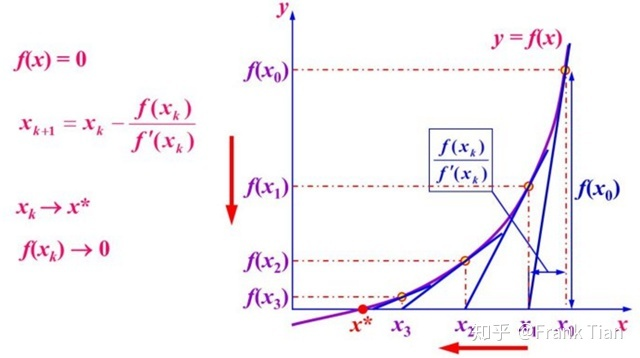
\includegraphics[scale=0.5]{newton.jpg}
%\end{figure}

(Algorithm 1.14. Newton’s method finds the root of $f : R \rightarrow R$ near an initial guess $x_0$ by the iteration formula)

\textbf{定理1.15(牛顿法的收敛性)。考虑 $B=[\alpha - \delta,\alpha - \delta]$上的函数 $f: B \rightarrow R$ ($f \in C^2$)满足 $f(\alpha) = 0$ 和 $f'(\alpha) \ne 0$。 如果选取的 $x_0$ 充分接近 $\alpha$,则牛顿方法中的迭代序列 $\{x_n\}$ 二次收敛到根 $\alpha$,即:}

(Theorem 1.15 (Convergence of Newton’s method). Consider a $C^2$ function $f : B \rightarrow R$ on $B = [\alpha − \delta, \alpha + \delta]$ satisfying $f(\alpha) = 0$ and $f'(\alpha) \ne 0$. If $x_0$ is chosen sufficiently close to $\alpha$, then the sequence of iterates ${x_n}$ in the Newton’s method converges quadratically to the root $\alpha$, i.e.)

\[
\lim_{n \rightarrow \infty}
\frac{\alpha - x_{n+1}}{(\alpha - x_n)^2} = -\frac{f''(\alpha)}{2f'(\alpha)}. (1.8)
\]

\textbf{证明. 根据泰勒定理(定理C.60)和所假设的函数 $f(f \in C^2)$, 我们有}

(Proof. By Taylor’s theorem (Theorem C.60) and the assumption $f \in C^2$, we have)

\[
f(\alpha) = f(x_n) + (\alpha - x_n)f'(x_n) + \frac{(\alpha - x_n)^2}{2}f''(\xi)
\]

\textbf{当 $\xi$ 在 $\alpha$ 和 $x_n$ 之间, $f(\alpha) = 0$ 得:}

(When $\xi$ is between $\alpha$ and $x_n$. $f(\alpha)) = 0$ yields)

\[
-\alpha = -x_n + \frac{f(x_n)}{f'(x_n)} + \frac{(\alpha - x_n)^2}{2} \frac{f''(\xi)}{f'(x_n)}.
\]

\textbf{通过式子(1.7), 我们有:}

(By (1.7), we have)

\[
(*): x_{n+1} - \alpha = x_n - \frac{f(x_n)}{f'(x_n)} - \alpha = (x_n - \alpha)^2\frac{f''(\xi)}{2f'(x_n)}.
\]

\textbf{通过 $f'$ 的连续性以及 $f'(\alpha) \ne 0$的假设:}

(The continuity of $f'$ and the assumption $f'(\alpha) \ne 0$ yield)

\[
\exists \delta _1 \in (0,\delta) s.t. \forall x \in B_1, f'(x) \ne 0
\]

\textbf{其中 $B_1 = [\alpha-\delta _1, \alpha + \delta _1]$. 定义:}

(Where $B_1 = [\alpha-\delta _1, \alpha + \delta _1]$. Define )

\[
M = \frac{max_{x \in B_1}|f''(x)|}{2min_{x \in B_1}|f'(x)|}
\]

\textbf{选取 $x_0$, 使它接近 $\alpha$, 使得:}

(And pick $x_0$ sufficiently close to $\alpha$ such that)

(i) $|x_0 - \alpha| = \delta_0 \le \delta_1$;

(ii) $M \delta_0 \le 1$.

\textbf{由 M 和 (*) 的定义有:}

(The definition of M and (*) imply)

\[
|x_{n+1} - \alpha| \le M|x_n - \alpha|^2.
\]

\textbf{将上述与不等式与(1.3)进行比较可得, 如果 $\{x_n\}$ 收敛,则收敛阶数为2。我们仍然必须证明 (a) 它收敛, 并且(b) 它收敛到 $\alpha$。}

\textbf{通过 (i) 和 (ii), 我们有 $M|x_0 − \alpha| < 1$。 然后通过归纳可以很容易获得以下结果:}

\[
|x_n - \alpha| \le \frac{1}{M}(M|x_0 - \alpha|)^{2^n},
\]

\textbf{这说明了 (a) 和 (b), 且完成了证明.}

(Comparing the above to (1.3) implies that if $\{x_n\}$ converges, then the order of convergence is 2. We must still show that (a) it converges and (b) it converges to $\alpha$.)

(By (i) and (ii), we have $M |x_0 − \alpha| < 1$. Then it is easy to obtain the following via induction, which shows both (a) and (b) and completes the proof.)


\section{Polynomial Interpolation 多项式插值}
\section{Splines 样条}
\section{Computer Arithmetic 计算机算法}
\section{Approximation 近似值}
\section{Numerical Integration and Differentiation 数值积分与微分}
\section{附录}

\end{document}
